\documentclass{article}
\usepackage[UTF8]{ctex}
\usepackage{geometry}
\usepackage{multirow}
\usepackage{natbib}
\geometry{left=3.18cm,right=3.18cm,top=2.54cm,bottom=2.54cm}
\usepackage{graphicx}
\pagestyle{plain}	
\usepackage{setspace}
\usepackage{enumerate}
\usepackage{caption2}
\usepackage{float}
\usepackage{datetime} %日期
\renewcommand{\today}{\number\year 年 \number\month 月 \number\day 日}
\renewcommand{\captionlabelfont}{\small}
\renewcommand{\captionfont}{\small}
\begin{document}

\begin{figure}
    \centering
    
\includegraphics[width=8cm]{upc.png}

    \label{figupc}
\end{figure}

	\begin{center}
		\quad \\
		\quad \\
		\heiti \fontsize{45}{17} \quad \quad \quad 
		\vskip 1.5cm
		\heiti \zihao{2} 《计算科学导论》个人职业规划
	\end{center}
	\vskip 2.0cm
		
	\begin{quotation}
% 	\begin{center}
		\doublespacing
		
        \zihao{4}\par\setlength\parindent{7em}
		\quad 

		学生姓名:\underline{\qquad 孙百乐 \qquad \qquad}

		学\hspace{0.61cm} 号:\underline{\qquad 2007010218\qquad}
		
		专业班级:\underline{\qquad 人工智能2001 \qquad  }
		
        学\hspace{0.61cm} 院:\underline{计算机科学与技术学院}
% 	\end{center}
		\vskip 1.5cm
		\centering
		\begin{table}[h]
            \centering 
            \zihao{4}
            \begin{tabular}{|c|c|c|c|c|c|c|c|c|}
            % 这里的rl 与表格对应可以看到,姓名是r,右对齐的;学号是l,左对齐的;若想居中,使用c关键字。
                \hline
                \multicolumn{5}{|c|}{分项评价} &\multicolumn{2}{c|}{整体评价}  & 总    分 & 评 阅 教 师\\
                \hline
                自我 & 环境 & 职业 & 实施 & 评估与 & 完整性 & 可行性 &\multirow{2}*{} &\multirow{2}*{}\\
                分析& 分析& 定位 & 方案 & 调整 & 20\% & 20\% & ~&~ \\\            
                10\% & 10\% & 15\% & 15\% & 10\% & &  &~ &~\\
                \cline{1-7} 
                & & & & & & & ~&~ \\
                & & & & & & & ~&~ \\
                \hline      
            \end{tabular}
        \end{table}
		\vskip 2cm
		\today
	\end{quotation}

\thispagestyle{empty}
\newpage
\setcounter{page}{1}
% 在这之前是封面,在这之后是正文
\section{自我分析}
	我已经和自己相处了19年,我应该很了解自己,而且我也不会有本质的改变了。所以这篇职业规划的核心内容就是自我分析。
	自我分析包括:
\subsection{自然条件}
姓名孙百乐,性别男,年龄19岁,身高略高,体重正常,身体健康,故乡在安徽蚌埠,现在山东省青岛市黄岛区中国石油大学(华东)上大学。\par
\subsection{性格分析}
我的性格偏内向,在人际交往中比较被动,公共场合不喜多言,不擅长和老师,长辈,上级领导等打交道。对不熟悉的人我话不多,但是熟悉之后,能很快形成友谊,建立信任,并让别人发现我其实很有趣。我的这种性格可以概括成“闷骚”(我不认为这是一个贬义词)。我是一个率真坦直的人,我喜欢和我一样踏踏实实的人,讨厌弄虚作假,表里不一,反复不定的人。但是偶尔我也会在意外表,追求虚荣,经常会在意别人的看法。我的三观比较端正,思想以传统儒家道德为主,不太开放。我的性格比较乐观,经常以积极的眼光看待已经发生的事情。我责任心较强,对待自己的事情,我神经大条,不太在意(这也是一种缺点),但如果是别人托付给我的任务,我会感到有压力,认真对待。同龄人评价我比较稳重,遇事沉着冷静,即使内心慌张,表面也能波澜不惊。我也常多愁善感,在心里臧否人事,但多不表露。\par
\begin{figure}[H]
	\centering
	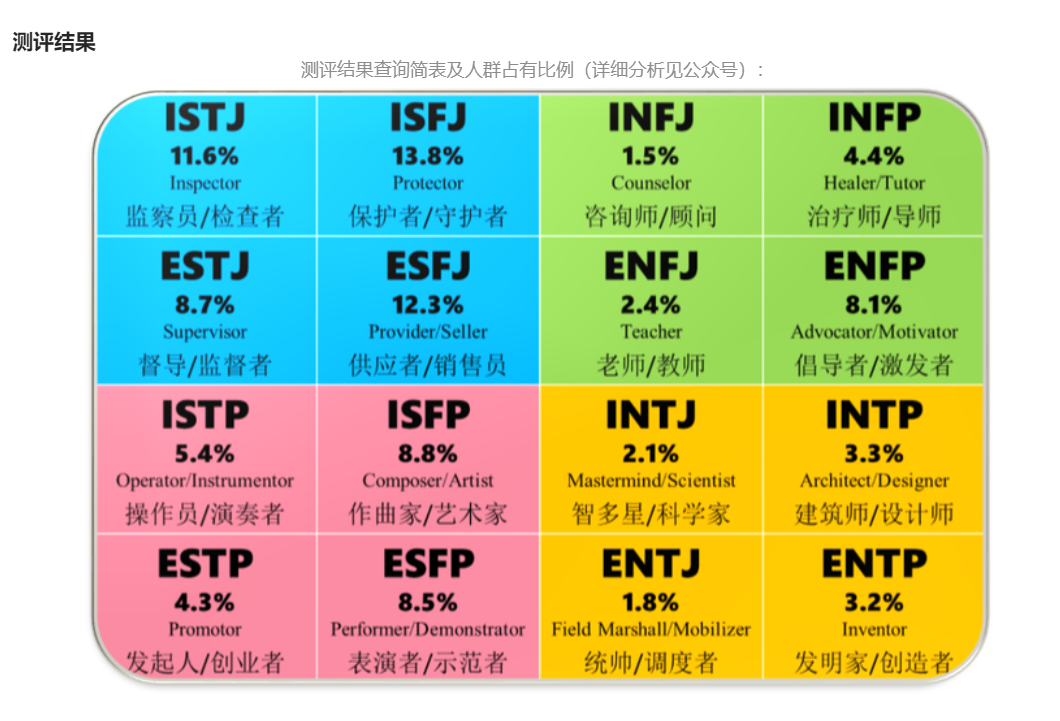
\includegraphics[width=0.8\linewidth]{性格测试1}
	\caption{}
	\label{fig:1}
\end{figure}
\begin{figure}[H]
	\centering
	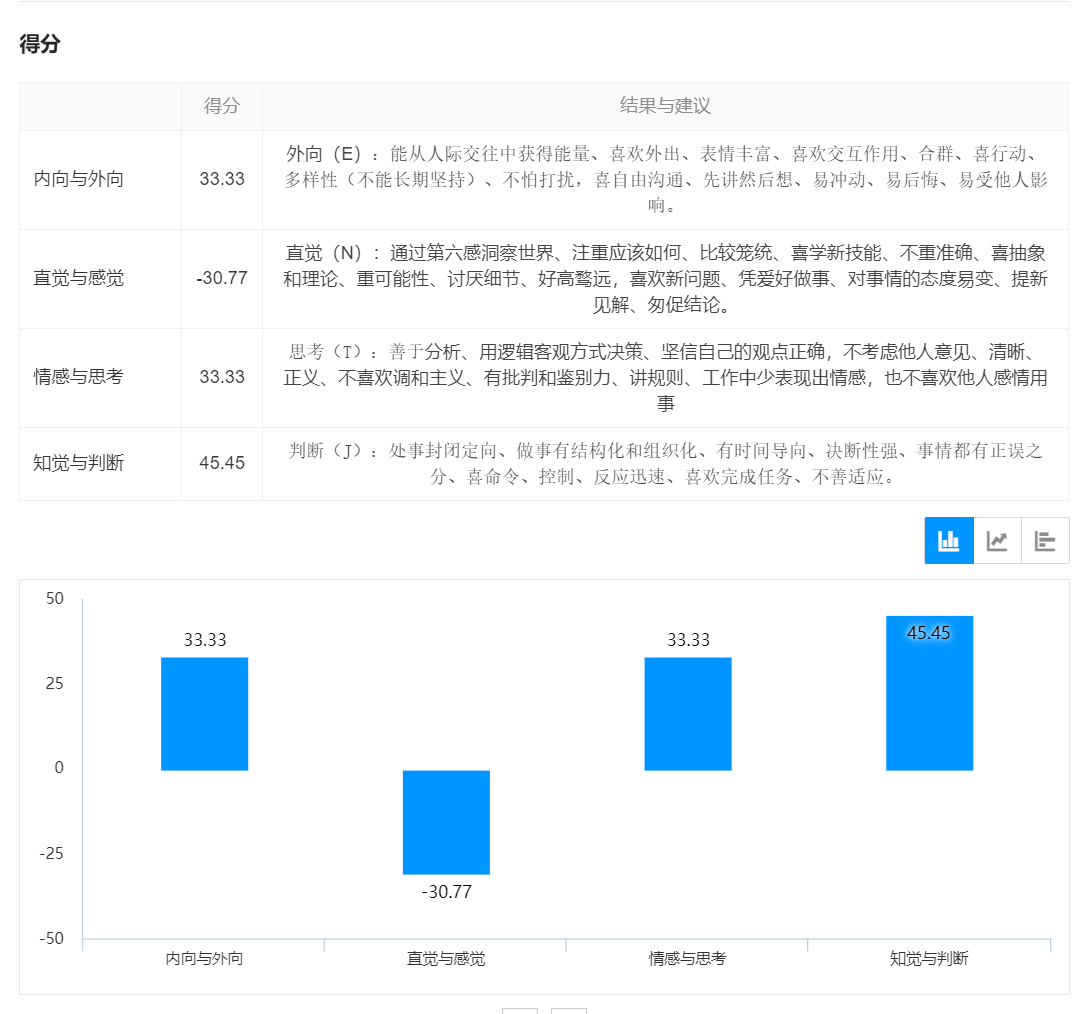
\includegraphics[width=0.8\linewidth]{性格测试2}
	\caption{}
	\label{fig:2}
\end{figure}


\subsection{教育与学习经历}
小学,初中,高中都在蚌埠本地上学,受到的教育比较单一。从小对电脑感兴趣,其它方面没什么才艺。\par
上大学后,兴趣比较广泛,喜欢阅读,政治,经济,文化(尤其是地理文化差异)等方面的书籍都有看。暑假学习了吉他,对音乐也有兴趣。在大学,老师鼓励关注最新学术动态,使我的视野比较开阔。感觉未来我可以有无限可能。\par
从小到大,成绩是比较优异,数理基础不差。但很缺乏社会实践。
\subsection{工作与社会阅历}
没有参加过工作,社会阅历基本与同龄人相当。\par
\subsection{知识、技能与经验}
与同龄人相比,了解知识比较广泛,具备技能也比较多,如篮球,排球,吉他,唱歌,滑板,做视频,做ppt,使用电脑等。能熟练使用解决问题。\par
另外我具有一定的领导力,在小组中,我能吸收各成员的建议,了解各成员的想法,我会对团体负责,我经常会成为最终决策者。\par
我喜欢阅读,在读书的时候经常会有创意想法,并渴望去实践,因此我觉得我具有一定的创新能力。\par
\subsection{兴趣爱好与特长}
爱好较广泛,前面已经有提到,特长是对跟电脑,网络有关的新生事物理解力比较强。\par
\subsection{霍兰德职业测评}
职业兴趣的整体概况:
\begin{figure}[H]
	\centering
	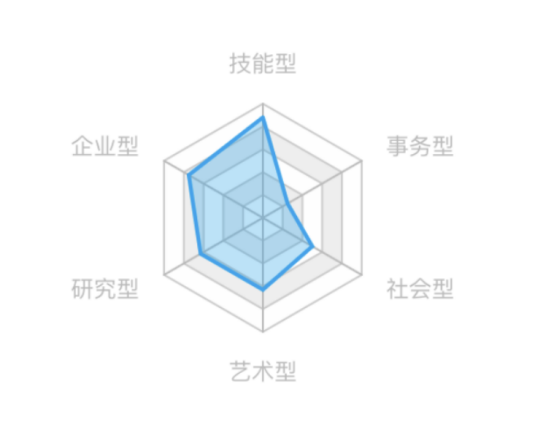
\includegraphics[width=0.7\linewidth]{图片1}
	\caption{}
	\label{fig:1}
\end{figure}

兴趣类型:技能型
兴趣类型:
技能型(R)
类型解释:
愿意使用工具从事操作性工作,动手能力强,做事手脚灵活,动作协调。偏好于具体任务,不善言辞,做事保守,较为谦虚。缺乏社交能力,通常喜欢独立做事。喜欢使用工具、机器,需要基本操作技能的工作。对要求具备机械方面才能、体力或从事与物件、机器、工具、运动器材、植物、动物相关的职业有兴趣,并具备相应能力。
适合职业:
技术性职业(计算机硬件人员、摄影师、制图员、机械装配工),技能性职业(木匠、厨师、技工、修理工、农民、一般劳动)\par
兴趣类型:
企业型(E)
类型解释:
追求权力、权威和物质财富,具有领导才能。喜欢竞争、敢冒风险、有野心、抱负。为人务实,习惯以利益得失,权利、地位、金钱等来衡量做事的价值,做事有较强的目的性。喜欢要求具备经营、管理、劝服、监督和领导才能,以实现机构、政治、社会及经济目标的工作,并具备相应的能力。
适合职业:
项目经理、销售人员,营销管理人员、政府官员、企业领导、法官、律师\par
兴趣类型:
研究型(I)
类型解释:
思想家而非实干家,抽象思维能力强,求知欲强,肯动脑,善思考,不愿动手。喜欢独立的和富有创造性的工作。知识渊博,有学识才能,不善于领导他人。考虑问题理性,做事喜欢精确,喜欢逻辑分析和推理,不断探讨未知的领域。喜欢智力的、抽象的、分析的、独立的定向任务,要求具备智力或分析才能,并将其用于观察、估测、衡量、形成理论、最终解决问题的工作,并具备相应的能力。
适合职业:
科学研究人员、教师、工程师、电脑编程人员、医生、系统分析员。\par
\section{环境分析}
环境分析主要是评估周边各种环境因素对自己职业生涯发展的影响。每一个人都处在一定的环境之中,职业发展必然要受到所处环境的影响,只有充分了解和把握所处环境的现状、特点、发展变化趋势,才能做到在复杂的环境中避害趋利,使你的职业生涯规划具有实际意义。\par
环境分析包括:\par
\subsection{社会环境分析}
现阶段,疫情给就业造成巨大压力,但同时也加速了互联网行业的发展。估计等我毕业时,疫情完全结束,就业恢复稳定。\par
近几年国家的战略发展离不开计算机。国家鼓励全民学计算机,计算机科学与技术号称“宇宙第一专业”,社会对计算机从业人员还是很尊重的。\par
目前互联网行业发展的趋势是,各行各业都在往互联网靠拢,与互联网融合。互联网内部也会出现很多新产品,以后的就业机会还是比较多的。\par


\subsection{家庭环境分析}
父母都有稳定的工作,父亲是公务员,母亲是社会工作者,家里经济条件稳定。家人比较期望我未来能有稳定的工作,过小日子。\par
未来如果我遭遇挫折,家庭可以成为我的避风港。\par
\subsection{职业环境分析}
从业人员多为男性,工作形式比较普遍的是程序员,如果进大厂的话工作环境很不错,工作较为辛苦,脑力活动多人际交流偏少,工资高。\par
计算机相当热门,从业人员很多。但高水平人才仍缺少。计算机要求技术人才较多,理论人才需求较少,技术更迭较快,学计算机考研的较少,更多人会趁着年轻去找工作,竞争比较激烈。\par
近年来,计算机专业已经不是当今社会的主流。接目前软件产业的发展速度来看,在未来的三到五年内,共需要软件开发人员两到三万人,其中急需三类人才:第一类是既懂技术又懂管理的软件件高级人オ;第二类是系统分析及设计人员,即软件工程师;第三类是熟练的程序员,即软件蓝领。\par

\subsection{地域与人际环境分析}
一线城市如北上广深,机会更多。但我更喜欢青岛,因为很喜欢青岛美丽的风景,喜欢好客的山东人。青岛也是新一线城市,虽然比不上北上广深,但也有很多机会。\par
家乡是蚌埠市,是安徽第三大城市,商业比较发达。家里在蚌埠熟人较多,我在蚌埠找一份像样的工作也不难。\par


\section{职业定位}
我现在是大一,对职业定位还很模糊,且非常感性,所以职业定位可能并不准确,但是能一定程度上代表我内心的想法,以后会再作修改。\par
职业定位包括:\par

\subsection{行业领域定位与理由}
想进入计算机与互联网行业。理由:1.有兴趣。2.行情好,国家支持。3.能赚钱。\par
\subsection{职业岗位起点定位与理由}
职业起点一:毕业后与同学一起创业,可以从工作室,小作坊做起。职业起点二:面试进大厂。职业起点三:考公务员。\par
理由:作为普通大学生,毕业后起点不可能太高,仍需要继续学习技能,并接触更多优秀的人,去遇见更多机会。
\subsection{职业目标与可行性分析}

成果目标、经济目标、能力目标、职务目标等。
\begin{enumerate}[(1)]
	\item 短期目标(大学4年)打好数理基础(尤其是学好数学),打好专业基础。我对计算机软件和硬件都没有偏执,我更喜欢软硬结合地做一些综合项目。要成为系统性人才,要像鲶鱼一样可以自由在前端后端,软件硬件之间遨游。
	\item 中长期目标(5-10年)。在计算机的某个领域成为专家,做到国内一流,然后升到管理层。做CTO。
\end{enumerate}
\begin{itemize}
    \item 目标职业一:创业做产品,成为下一个乔布斯。可行性分析:基本不可能。
    \item 目标职业二:成为大公司的CTO。可行性分析:通过努力,有可能。
    \item 目标职业三:做自媒体,与他人合作成立工作室。可行性分析:可能性比较大。
    \item 目标职业四:回老家,考公务员,或找其它稳定的工作。可行性分析:如果前面三个都没有机遇的话再选择这个。实现可能性比较大。
\end{itemize}


\section{实施方案}
在明确了职业定位后,要制定实现职业生涯目标的行动方案,不付诸行动,职业目标只能是一种梦想。实施方案是实现职业目标的保证,尽量考虑周全、具有可操作性。\par


 \subsection{如何利用现有条件和自身优势以实现职业生涯目标?}
 \begin{enumerate}
 \item 本科阶段尽量多学一些技能,比如会计,管理等,同时把本专业的知识学好。
 \item 多与导师交流,参加大创等活动,争取在学校里把一个大项目做成功,拿到奖。其它的小项目多做。
\item 提升判断力,学会洞察行情,自己多总结,然后和大牛多交流。
 \end{enumerate}
  \subsection{如何克服缺点、弥补不足、增长知识、提高能力以实现职业生涯目标?}
 \begin{enumerate}
 	\item 使用好github这个平台,以及多看b站上一些程序员大牛分享的经验。
 	\item 多读书,养成“不可一日无书”的习惯。
 	\item 多出去走一走,观察青岛的风土人情,以及就业情况。
 	\end{enumerate}
  \subsection{如何处理人际关系和发展人脉以实现职业生涯目标?}
 \begin{enumerate}
\item 在社团中担当职位,多与人接触交流,克服社交恐惧。
\item 有空写一些文章发在班级站点上,提升写作技能。
 \end{enumerate}
  \subsection{如何处理工作与家庭、生活的关系以实现职业生涯目标?}
 \begin{enumerate}
\item 与家里人保持联系,把生活照片发给家里人,让家里人了解我的大学生活。
 \end{enumerate}
 \subsection{ 如何处理释放工作压力、保证身心健康以实现职业生涯目标?}
\begin{enumerate}
	\item 假期把吉他学好,能弹喜欢的歌,释放压力。多打篮球,认识一些球友。
\end{enumerate}
在网上找到了一张CTO技能图谱,参考性很强。
\begin{figure}[H]
	\centering
	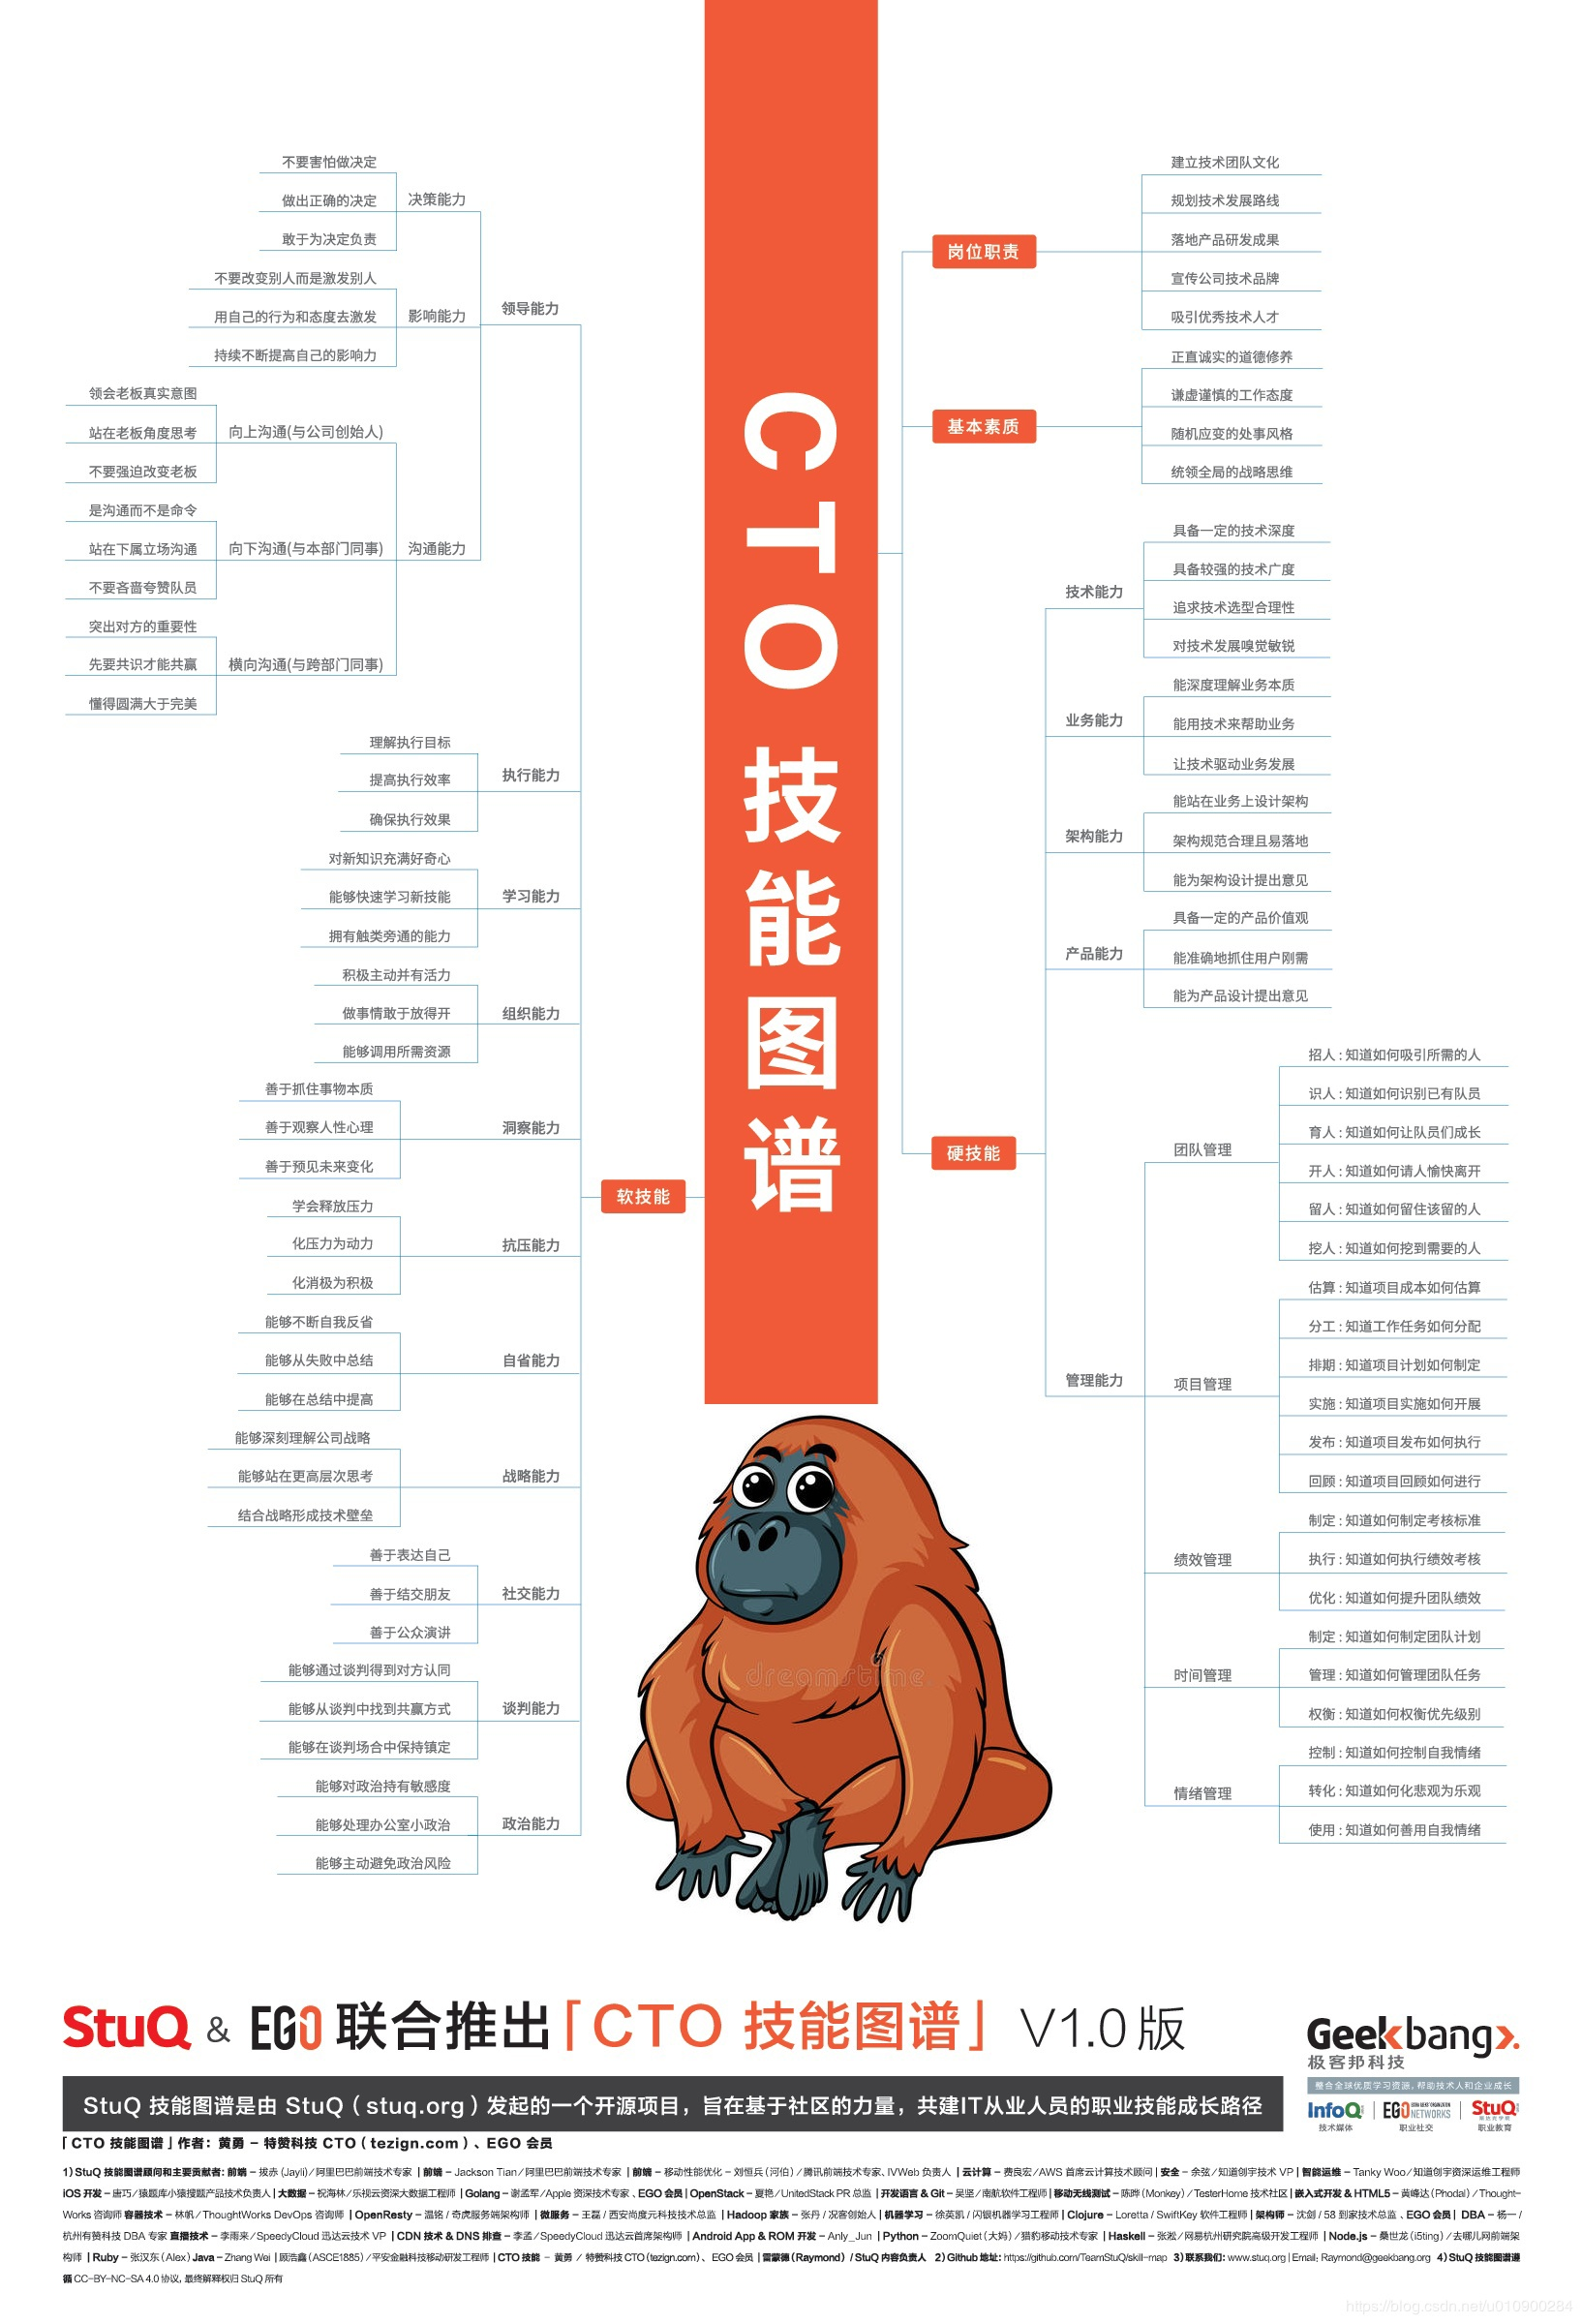
\includegraphics[width=1\linewidth]{skillmap}
	\caption{CTO技能图谱}
	\label{fig:skillmap}
\end{figure}
\section{评估与调整}
影响职业生涯规划的因素很多,且大都处于动态变化之中,因此职业生涯规划应定期评估,并根据影响因素的变化和实施结果的情况及时作出调整,这样才能保证其行之有效。\par 
我知道现在自己看待未来就仿佛是身处大雾之中,一片朦胧。但我会一直往前走,路漫漫其修远兮,吾将上下而求索。\par 
\subsection{评估时间}
每学年评估一次,每次评估时间为每年12月25日。\par
\subsection{评估内容}
完成下表,并写一篇年度总结。\par
\begin{table}[h]
	\centering
	\begin{tabular}{|l|l|l|l|l|}
		\hline
		& \textbf{成绩目标} & \textbf{能力目标} & \textbf{职务目标} & \textbf{阅读目标} \\ \hline
		已完成  &               &               &               &               \\ \hline
		未完成  &               &               &               &               \\ \hline
		需要修改 &               &               &               &               \\ \hline
	\end{tabular}
\end{table}
\subsection{调整原则}
\begin{itemize}
	\item 尽量考虑长远,尽量与时俱进。
	\item 不能立志做违反法律,违反道德,违背国家的事情。
\end{itemize}




\end{document}
